\section{Theoretical Models}

\subsection{Capital Asset Pricing Model (CAPM)}
The Capital Asset Pricing Model (CAPM) is a fundamental tool in finance used to determine the expected return on an asset based on its systematic risk, as measured by beta ($\beta_i$). The CAPM formula is:

\begin{equation}
E(R_i) = R_f + \beta_i(E(R_m) - R_f)
\end{equation}

where:
\begin{itemize}
    \item $E(R_i)$ is the expected return on asset $i$.
    \item $R_f$ is the risk-free rate of return.
    \item $\beta_i$ is the beta of asset $i$, representing its sensitivity to market movements.
    \item $E(R_m)$ is the expected return of the market.
    \item $(E(R_m) - R_f)$ is the market risk premium.
\end{itemize}

\subsubsection{Beta Calculation}
Beta ($\beta_i$) measures the volatility of an asset in relation to the market. It is calculated as:

\begin{equation}
\beta_i = \frac{\text{Cov}(R_i, R_m)}{\sigma^2_m}
\end{equation}

where:
\begin{itemize}
    \item $\text{Cov}(R_i, R_m)$ is the covariance between the return of asset $i$ and the return of the market.
    \item $\sigma^2_m$ is the variance of the market return.
\end{itemize}
This model is crucial for understanding the risk-return tradeoff and is widely used in portfolio management \citep{fama1973risk}.

\subsubsection{Security Market Line (SML)}
The Security Market Line (SML) is a graphical representation of the CAPM, showcasing the relationship between the expected return of an asset and its systematic risk, as measured by beta ($\beta_i$).

\begin{figure}[!ht]
    \centering
    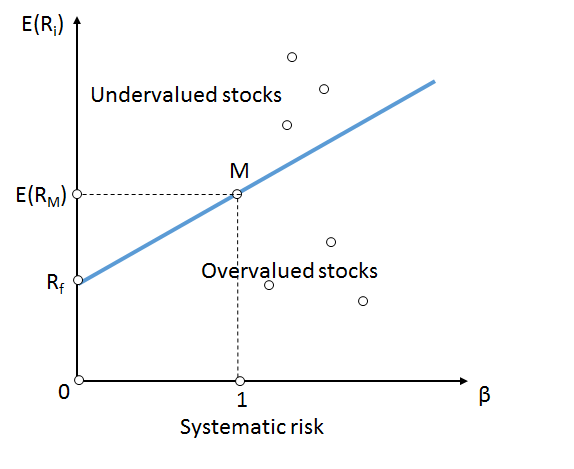
\includegraphics[width=0.6\textwidth]{../Figures/SML.png}
    \caption{Security Market Line}
    \label{fig:SML}
    \subcaption{Illustrates the Security Market Line (SML), which plots the expected return of an asset against its beta. The SML demonstrates that assets with higher systematic risk (higher beta) should offer higher expected returns to compensate for the increased risk.}
\end{figure}

\subsubsection{Theoretical Implications}
The SML conveys several important theoretical implications:
\begin{itemize}
    \item All securities, when correctly priced, should lie on the SML.
    \item The slope of the SML is the market risk premium, $E(R_m) - R_f$, representing the additional return expected from holding a market portfolio instead of risk-free assets.
    \item The intercept of the SML is the risk-free rate, $R_f$, reflecting the return of a theoretically risk-free asset \citep{sharpe1964capital}.
\end{itemize}

\subsection{Sharpe Ratio}
The Sharpe Ratio, developed by William F. Sharpe, is a measure of risk-adjusted return. It is calculated as follows:

\begin{equation}
\text{Sharpe Ratio} = \frac{E(R_i) - R_f}{\sigma_i}
\end{equation}

where:
\begin{itemize}
    \item $E(R_i)$ is the expected return of the investment.
    \item $R_f$ is the risk-free rate.
    \item $\sigma_i$ is the standard deviation of the investment's return.
\end{itemize}

\subsubsection{Interpretation}
The Sharpe Ratio provides a way to compare the performance of investments while considering the risk taken. A higher Sharpe Ratio indicates better risk-adjusted performance, meaning the investment provides higher returns for each unit of risk taken \citep{sharpe1966mutual}.

\subsection{Composite Score Calculation}
The Composite Score integrates multiple metrics to rank securities. It is calculated as follows:

\begin{equation}
\text{Composite Score} = w_{\beta} \beta + w_{\text{Sharpe}} \text{Sharpe Ratio} + w_{\text{CAPM}} E(R_i) + w_{\text{Actual}} \text{Actual Returns}
\end{equation}

where:
\begin{itemize}
    \item $w_{\beta}$ is the weight assigned to the beta.
    \item $w_{\text{Sharpe}}$ is the weight assigned to the Sharpe Ratio.
    \item $w_{\text{CAPM}}$ is the weight assigned to the CAPM predicted return.
    \item $w_{\text{Actual}}$ is the weight assigned to the actual returns.
\end{itemize}

Weights are assigned to each metric to reflect their importance in the ranking process.

\subsection{Modern Portfolio Theory (MPT)}
Modern Portfolio Theory (MPT), developed by Harry Markowitz, \citep{markowitz1952portfolio} provides a robust framework for constructing an optimal portfolio that maximizes expected return for a given level of risk. The expected return $E(R_p)$ of a portfolio is the weighted sum of the expected returns of the individual assets:

\begin{equation}
E(R_p) = \sum_{i=1}^n w_iE(R_i)
\end{equation}

where:
\begin{itemize}
    \item $E(R_p)$ is the expected return of the portfolio.
    \item $w_i$ are the weights of the individual assets in the portfolio.
    \item $E(R_i)$ is the expected return of asset $i$.
\end{itemize}

\subsubsection{Efficient Frontier and Optimal Portfolio}
The efficient frontier is a concept from MPT that represents the set of optimal portfolios offering the highest expected return for a defined level of risk. The process of constructing the efficient frontier involves solving the following optimization problem:

\begin{equation}
\min \sum_{i=1}^n \sum_{j=1}^n w_i w_j \sigma_{ij}
\end{equation}

subject to:

\begin{equation}
\sum_{i=1}^n w_i = 1
\end{equation}

and

\begin{equation}
E(R_p) = \sum_{i=1}^n w_iE(R_i)
\end{equation}

where:
\begin{itemize}
    \item $\sigma_{ij}$ is the covariance between the returns of assets $i$ and $j$.
    \item $w_i$ and $w_j$ are the weights of assets $i$ and $j$ in the portfolio.
\end{itemize}

\begin{figure}[h!]
    \centering
    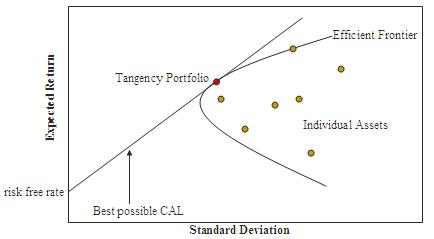
\includegraphics[width=0.6\textwidth]{../Figures/efficient_frontier.png}
    \caption{Efficient Frontier}
    \label{fig:efficient_frontier}
\end{figure}

\textbf{Explanation:} Figure \ref{fig:efficient_frontier} shows the efficient frontier, which illustrates the optimal portfolios that offer the maximum expected return for a given level of risk. Portfolios that lie below the efficient frontier are sub-optimal because they do not provide enough return for the level of risk taken \citep{markowitz1952portfolio}.

\subsection{Monte Carlo Simulation}
Monte Carlo simulations are utilized to model the uncertainty and variability in investment returns over time. The simulation process involves generating random returns based on historical data and iterating this process to build a distribution of potential outcomes. The value of an investment at time $i$ is given by:

\begin{equation}
X_i = X_{i-1} \times (1 + r_i)
\end{equation}

where:
\begin{itemize}
    \item $X_i$ is the investment value at time $i$.
    \item $X_{i-1}$ is the investment value at time $i-1$.
    \item $r_i$ is the return for period $i$.
\end{itemize}

By running multiple simulations, we can estimate the expected value and variability of the investment portfolio, providing insights into the likelihood of achieving the desired down payment amount within the specified time horizon \citep{glasserman2004monte}.

\begin{figure}[h!]
    \centering
    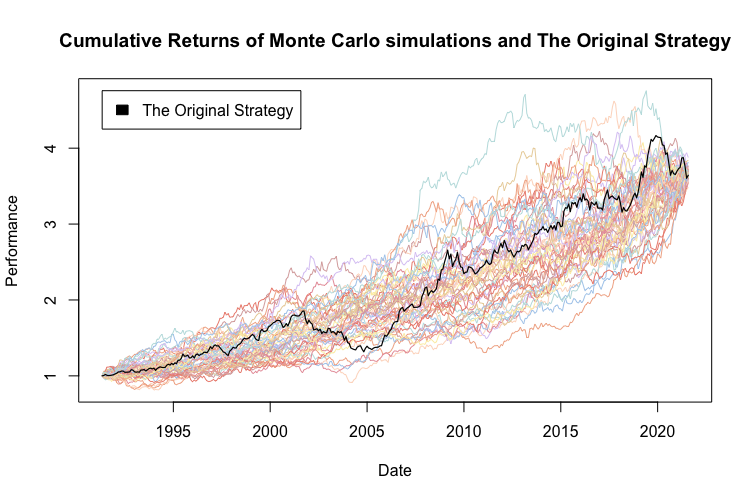
\includegraphics[width=0.6\textwidth]{../Figures/investment_simulation_process.png}
    \caption{Investment Simulation Process for Monte Carlo Analysis}
    \label{fig:investment_simulation}
\end{figure}

\textbf{Explanation:} Figure \ref{fig:investment_simulation} depicts the process of Monte Carlo simulation for investment analysis. The diagram shows how random returns are generated and used to project the future value of an investment over multiple iterations, creating a range of possible outcomes and helping to understand the potential risks and returns.

\newpage
